\documentclass[12pt,a4paper]{article}
\usepackage[utf8]{inputenc}
\usepackage{geometry}
\usepackage{graphicx}
\usepackage{amsmath}
\usepackage{hyperref}
\usepackage{titlesec}
\usepackage{changepage}
\usepackage{caption}
\usepackage{float}
\usepackage{booktabs}
\usepackage{tabularx}
\usepackage[numbers]{natbib} % Menambahkan paket natbib untuk referensi
\usepackage{setspace} % Untuk mengatur spasi antar baris
\usepackage{float} % Untuk mengontrol penempatan tabel
\usepackage{tabularx} % Untuk tabel dengan lebar yang dapat disesuaikan
\usepackage{booktabs}

% Page layout
\geometry{top=1in, bottom=1in, left=1in, right=1in}

% Modify section and subsection font size to normal
\titleformat{\section}[hang]{\normalsize\bfseries}{\thesection}{1em}{}
\titleformat{\subsection}[hang]{\normalsize\bfseries}{\thesubsection}{1em}{}

% Hanging indent for references
\setlength{\bibsep}{1em} % Mengatur jarak antar entri referensi
\setlength{\bibhang}{2em} % Mengatur indentasi menggantung untuk referensi

\begin{document}

% Title
\begin{titlepage}
    \centering
    {\Large\textbf{Deep Learning Course \\ Final Project Report}\par} % Judul
    \vspace{2cm} % Jarak antara judul dan logo
    
\includegraphics[width=0.5\linewidth]{Images/logounhas.png}\par % Logo
    \vspace{2cm} % Jarak antara logo dan nama
    {\large
    Trisman Tegar Wiratama (H071221023)\\ 
    Ammar Tyo Pasaribu (H071221079)\\ 
    Shaff Shalihin (H071221093)\par}
    \vspace{1cm} % Jarak antara nama dan tanggal
    {\large\today\par} % Tanggal
\end{titlepage}

\normalsize  % Set the text size to normal for the entire document
\tableofcontents
\newpage

% 1. Introduction
\section{INTRODUCTION}
\subsection{Latar Belakang dan Konteks Proyek}
\begin{adjustwidth}{3em}{0pt} 
\hspace{0.5cm} Pengelolaan sampah di lingkungan kampus merupakan tantangan serius yang dihadapi oleh institusi pendidikan tinggi, termasuk Universitas Hasanuddin. Setiap harinya, ribuan mahasiswa, dosen, dan staf menghasilkan berbagai jenis sampah yang membutuhkan penanganan yang tepat. Pemilahan sampah menjadi kategori organik dan anorganik merupakan langkah fundamental dalam sistem pengelolaan sampah yang efektif. Namun, proses pemilahan manual seringkali tidak konsisten dan membutuhkan waktu serta tenaga yang besar. Seiring dengan kemajuan teknologi, khususnya di bidang Deep Learning, klasifikasi sampah kini dapat dilakukan secara otomatis menggunakan model Convolutional Neural Network (CNN). Pendekatan ini menawarkan solusi yang lebih efisien dan akurat dalam mengidentifikasi jenis sampah, dibandingkan metode konvensional. \end{adjustwidth}
\

\subsection{Masalah}
\begin{adjustwidth}{3em}{0pt} 
\hspace{0.5cm} Kurangnya sistem pemilahan sampah yang efektif di lingkungan kampus menyebabkan tercampurnya sampah organik dan anorganik, yang mengakibatkan kesulitan dalam proses daur ulang dan pengomposan. Selain itu, belum tersedianya dataset sampah yang terorganisir dari lingkungan Universitas Hasanuddin menjadi kendala utama dalam pengembangan sistem otomatis berbasis kecerdasan buatan. Keterbatasan ini juga menghambat implementasi program pengelolaan sampah yang berkelanjutan di kampus. Tanpa adanya sistem klasifikasi yang akurat, efektivitas program reduce, reuse, dan recycle (3R) menjadi tidak optimal. \end{adjustwidth}

\subsection{Tujuan}
\begin{adjustwidth}{3em}{0pt} 
\hspace{0.5cm} Penelitian ini bertujuan untuk mengembangkan dataset komprehensif yang terdiri dari sampah organik dan anorganik yang dikumpulkan dari lingkungan Universitas Hasanuddin. Dataset ini akan digunakan untuk melatih model Deep Learning menggunakan dua arsitektur CNN yang berbeda, yaitu VGG16 dan ResNet, untuk mengklasifikasikan jenis sampah secara otomatis. Melalui perbandingan kedua arsitektur tersebut, penelitian ini berupaya mengidentifikasi model yang paling efektif dalam konteks klasifikasi sampah di lingkungan kampus. Lebih jauh lagi, penelitian ini bertujuan untuk mendukung program pengelolaan sampah kampus dengan menyediakan solusi teknologi yang dapat mengotomatisasi proses pemilahan sampah. Hasil dari penelitian ini diharapkan dapat menjadi landasan untuk pengembangan sistem pemilahan sampah otomatis yang dapat diimplementasikan di berbagai titik strategis di lingkungan kampus, sehingga mendukung terciptanya ekosistem kampus yang lebih berkelanjutan melalui pengelolaan sampah yang lebih efisien dan akurat.
\end{adjustwidth}

% \noindent Example:
% \lipsum[1] % Replace this with your content.

% 2. Related Works
\section{RELATED WORKS}
\begin{adjustwidth}{3em}{0pt}

\hspace{0.5cm} Klasifikasi otomatis sampah organik dan anorganik menggunakan teknik pembelajaran mendalam (deep learning) dan visi komputer (computer vision) telah menjadi fokus penelitian yang signifikan dalam upaya meningkatkan efisiensi pengelolaan sampah. Pendekatan berbasis deep learning telah menunjukkan hasil yang menjanjikan dalam mengidentifikasi dan mengklasifikasikan berbagai jenis sampah, terutama dengan tantangan variasi bentuk, warna, dan kondisi sampah yang kompleks. Kebutuhan akan sistem klasifikasi sampah yang efisien semakin meningkat seiring dengan pertumbuhan volume sampah global dan kesadaran akan pentingnya pengelolaan sampah yang berkelanjutan.

\vspace{1em}
\hspace{0.5cm} Penelitian awal oleh Rasidi et al. (2022) mengimplementasikan Convolutional Neural Network (CNN) untuk klasifikasi sampah organik dan anorganik. Dengan mencapai akurasi 85\%, penelitian ini membuktikan efektivitas CNN dalam memproses citra sampah. Metodologi yang digunakan melibatkan preprocessing gambar, augmentasi data, dan pelatihan model CNN dari awal. Meskipun hasil yang dicapai cukup menjanjikan, penelitian ini menghadapi tantangan dalam variasi dataset dan generalisasi model terhadap kondisi pencahayaan yang berbeda. Namun, penelitian ini menjadi landasan penting dalam pengembangan sistem klasifikasi sampah otomatis berbasis deep learning.

\vspace{1em}
\hspace{0.5cm} Terobosan signifikan dilakukan oleh Parasian (2022) yang mengembangkan pendekatan lebih canggih menggunakan arsitektur ResNet50 untuk klasifikasi sampah organik dan daur ulang. Penelitian ini mencapai hasil yang sangat memuaskan dengan akurasi pelatihan 99\% dan akurasi validasi 96\%. Keunggulan ResNet50 terletak pada kemampuannya mengatasi masalah vanishing gradient melalui skip connection, memungkinkan pelatihan jaringan yang lebih dalam dengan performa yang lebih baik. Metodologi yang diterapkan meliputi transfer learning dari model pre-trained pada ImageNet, fine-tuning pada dataset sampah, dan optimasi hyperparameter untuk meningkatkan performa model.

\vspace{1em}
\hspace{0.5cm} Kontribusi penting lainnya datang dari Fathurrahman (2024) yang memperkenalkan pendekatan berbasis transfer learning menggunakan TensorFlow Object Detection API. Penelitian ini mencapai Mean Average Precision (mAP) sebesar 0.858 dan Average Recall (AR) sebesar 0.91. Metodologi yang digunakan melibatkan penggunaan arsitektur pre-trained, modifikasi layer klasifikasi, dan implementasi teknik data augmentasi yang ekstensif. Meskipun mencapai hasil yang impresif, penelitian ini mengidentifikasi tantangan dalam generalisasi ke berbagai kondisi pencahayaan dan variasi sampah yang masih perlu diatasi.

\vspace{1em}
\hspace{0.5cm} Sunanto (2022) mengusulkan implementasi CNN dengan arsitektur yang lebih kompleks, menggunakan 128 lapisan dense dan pelatihan selama 50 epoch. Penelitian ini menerapkan teknik optimasi gradient descent yang disesuaikan dan regularisasi dropout untuk mencegah overfitting. Meskipun mencapai akurasi yang optimal pada data latih dan uji, keterbatasan utama penelitian ini terletak pada ukuran dataset yang relatif kecil (100 gambar). Hal ini menekankan pentingnya pengembangan dataset yang lebih besar dan beragam untuk meningkatkan robustness model.

\vspace{1em}
\hspace{0.5cm} Kemajuan dalam deteksi real-time ditunjukkan oleh Priana dan Karyawati (2023) yang mengimplementasikan metode YOLO untuk klasifikasi sampah, mencapai akurasi antara 80\% hingga 100\%. Penelitian ini menggabungkan teknik CNN dengan deteksi objek real-time, memungkinkan klasifikasi sampah secara langsung melalui video stream. Metodologi yang diterapkan meliputi penggunaan arsitektur YOLO yang dimodifikasi, augmentasi data real-time, dan optimasi untuk inferensi cepat. Kontribusi utama penelitian ini adalah demonstrasi kemungkinan implementasi sistem klasifikasi sampah dalam aplikasi dunia nyata.

\vspace{1em}
\hspace{0.5cm} Fantara et al. (2018) mengembangkan pendekatan berbeda menggunakan Jaringan Saraf Tiruan Backpropagation untuk klasifikasi sampah, mencapai akurasi 90\% dengan waktu pemrosesan rata-rata 42,9ms. Penelitian ini unik karena mengintegrasikan multiple sensor (LDR, proximity induktif, dan kapasitif) untuk meningkatkan akurasi klasifikasi. Meskipun efektif, pendekatan ini memiliki ketergantungan pada kondisi sensor yang dapat mempengaruhi reliabilitas sistem.

\vspace{1em}
\hspace{0.5cm} Dalam konteks penelitian ini, kami menggunakan dua arsitektur CNN populer - VGG16 dan ResNet - untuk klasifikasi sampah di lingkungan Universitas Hasanuddin. Pemilihan kedua arsitektur ini didasarkan pada keunggulan masing-masing: VGG16 dengan arsitektur yang sederhana namun powerful, dan ResNet dengan kemampuan mengatasi masalah vanishing gradient melalui skip connection. Dataset yang dikembangkan secara khusus dari lingkungan kampus memberikan konteks yang unik untuk evaluasi performa model dalam kondisi nyata.

\vspace{1em}
\hspace{0.5cm} Metodologi yang kami terapkan menggabungkan praktik terbaik dari penelitian sebelumnya, termasuk teknik preprocessing yang komprehensif, augmentasi data untuk meningkatkan variasi dataset, dan strategi transfer learning untuk mengoptimalkan performa model. Kami juga menerapkan teknik validasi silang dan evaluasi model yang ketat untuk memastikan reliabilitas hasil. Penggunaan dua arsitektur berbeda memungkinkan analisis perbandingan mendalam tentang kelebihan dan kekurangan masing-masing pendekatan dalam konteks klasifikasi sampah kampus.

\vspace{1em}
\hspace{0.5cm} Keunikan penelitian ini terletak pada fokusnya terhadap implementasi di lingkungan kampus, yang memiliki karakteristik sampah yang spesifik dan pola penggunaan yang berbeda dari lingkungan umum. Analisis komparatif antara VGG16 dan ResNet dalam konteks ini diharapkan dapat memberikan wawasan berharga untuk pengembangan sistem klasifikasi sampah yang lebih efektif di lingkungan akademik.

\end{adjustwidth}

% 3. Dataset and Material
\section{DATASET MATERIAL}
\subsection{Dataset}

Dalam proyek ini, kami membuat \textit{dataset} khusus untuk klasifikasi sampah organik dan anorganik di lingkungan Universitas Hasanuddin melalui langkah-langkah berikut:

\subsubsection{Sumber Dataset}
\begin{itemize}
    \item Foto Langsung: Gambar sampah diambil menggunakan kamera smartphone dari berbagai lokasi di lingkungan Universitas Hasanuddin untuk menangkap kondisi nyata sampah di kampus.
    \begin{figure}[h]
        \centering
        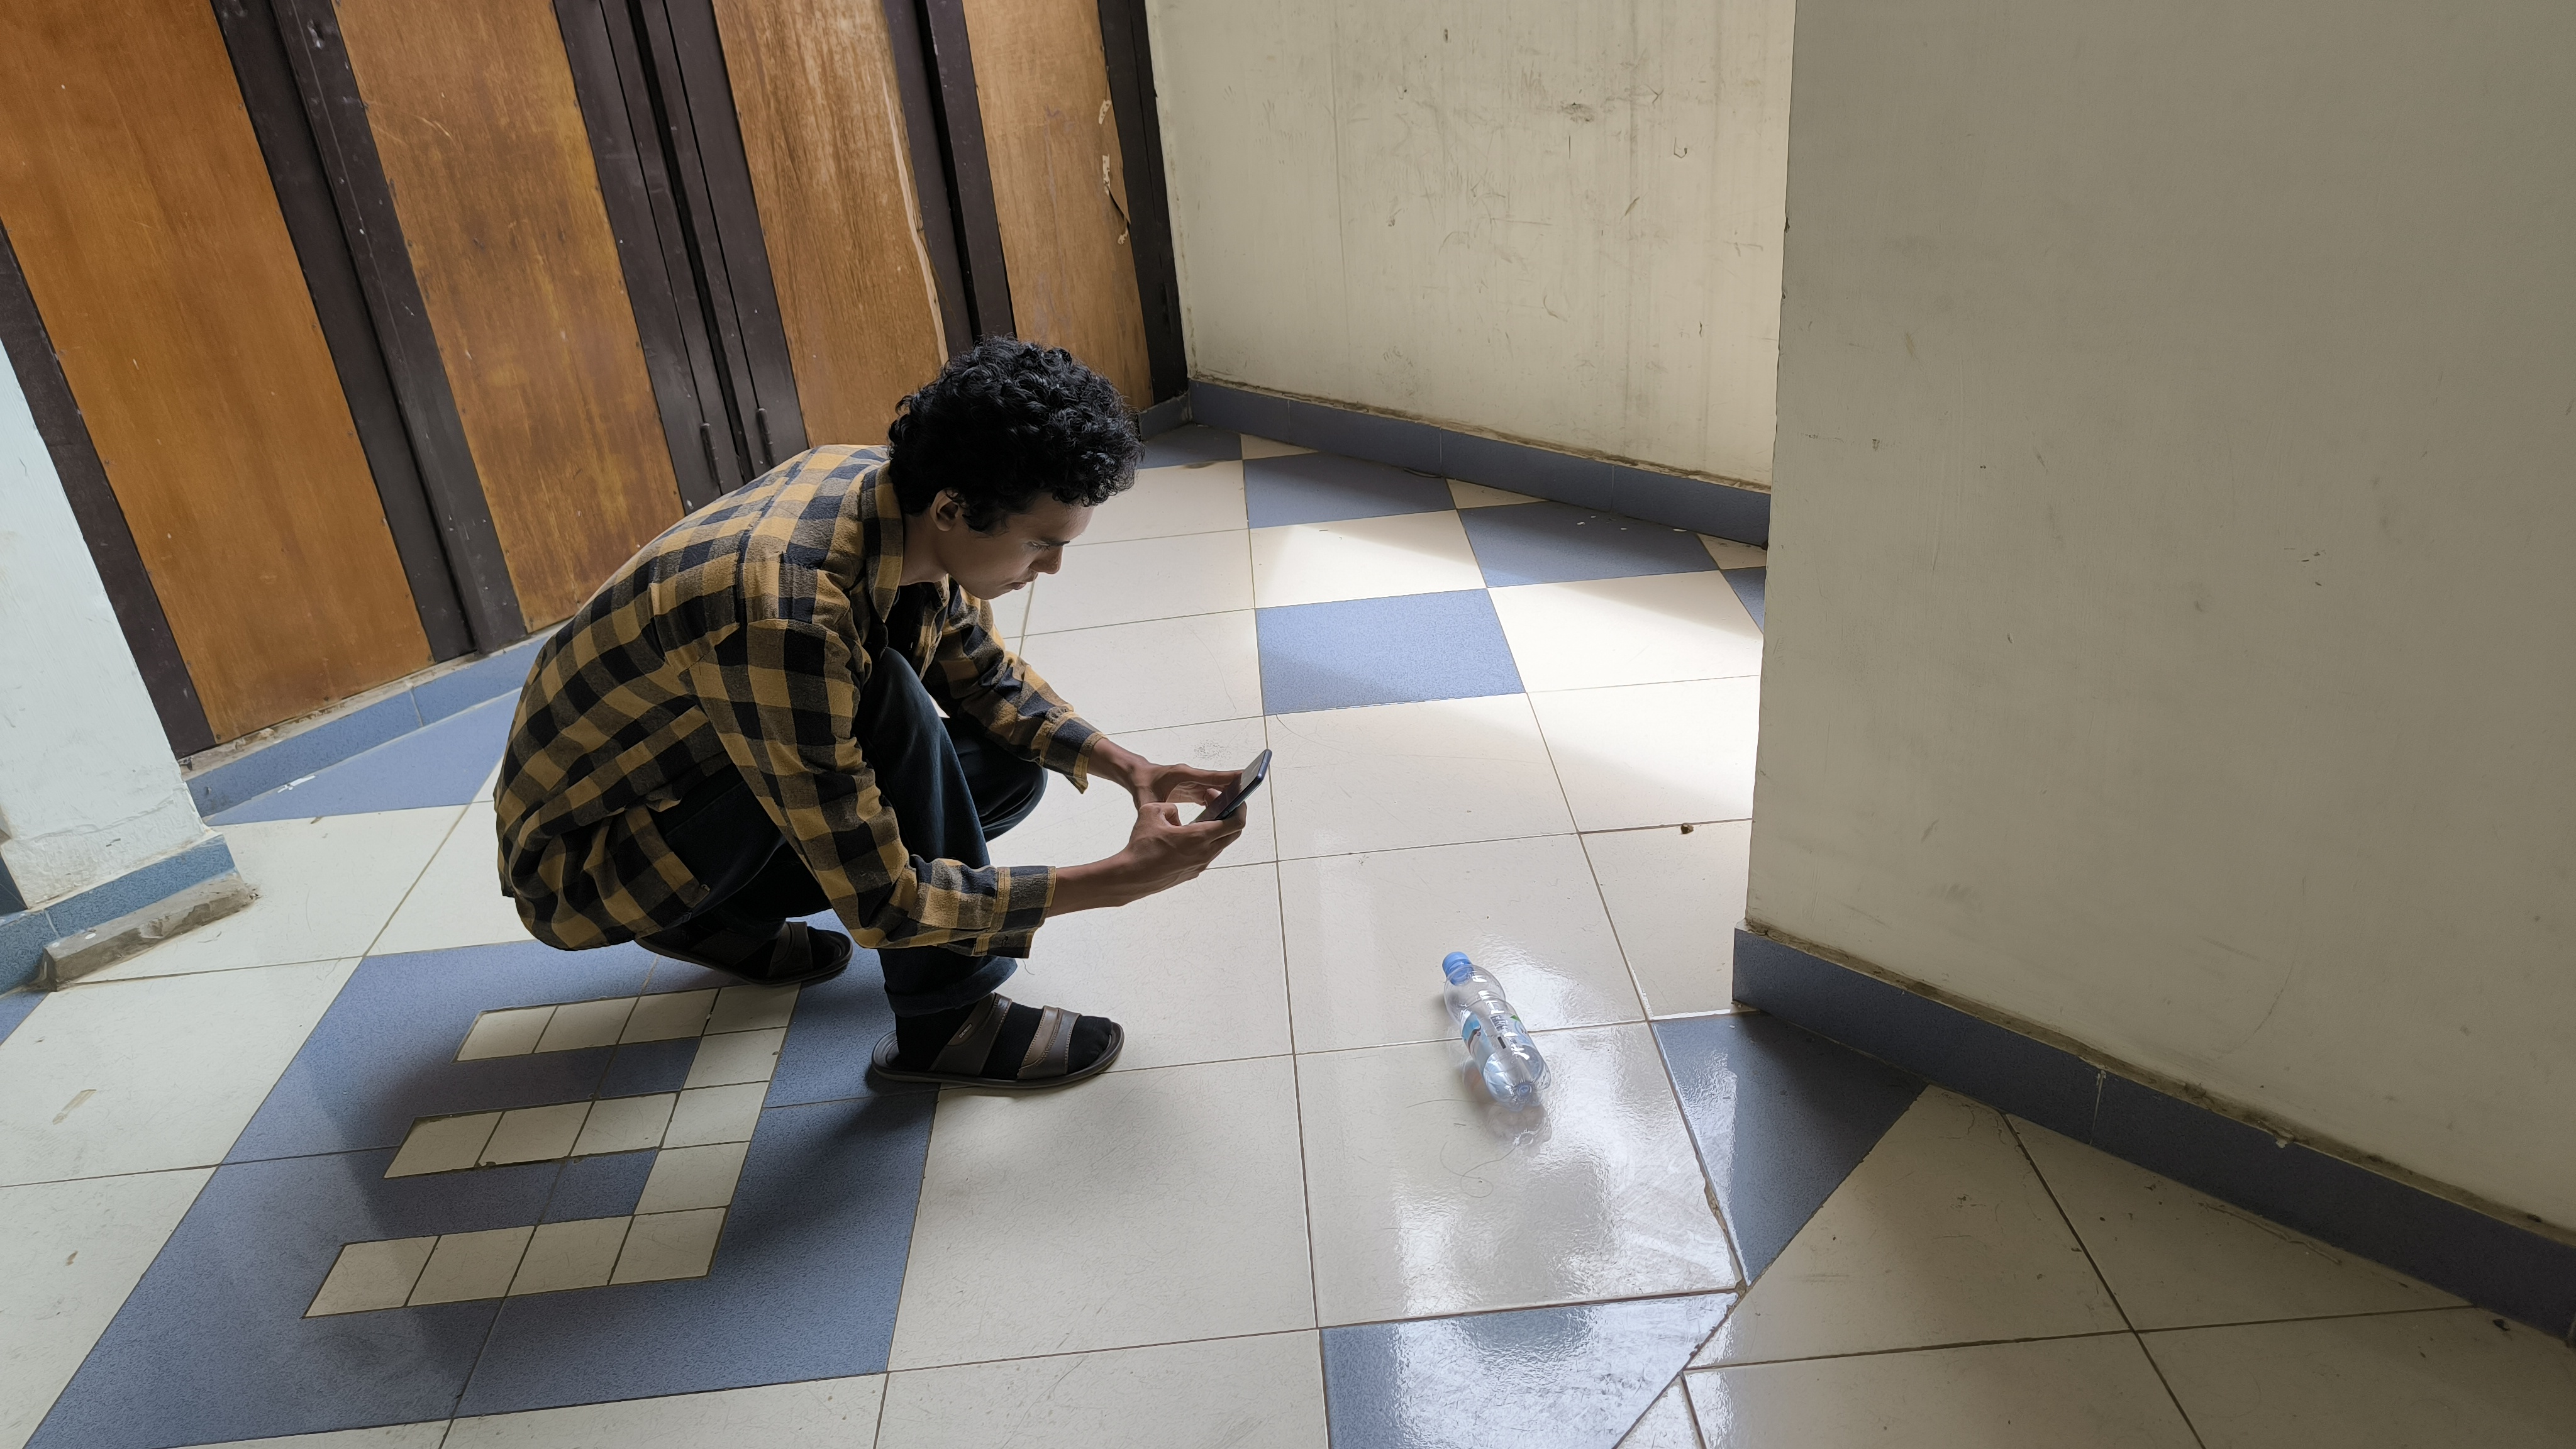
\includegraphics[width=0.6\linewidth]{Images/fotodataset.jpg}
        \caption*{Gambar 1. Pengambilan Gambar Sampah di Lingkungan Kampus}
        \label{fig:dataset_collection}
    \end{figure}
    
    \item Lokasi Pengambilan Data:
    \begin{itemize}
        \item Area Gedung PBT FMIPA Unhas
        \item Area Jasmip FMIPA Unhas
        \item Sekitaran Kudapan BNI
        \item Sekitaran Lapangan FMIPA Unhas
        
    \end{itemize}
    
    \item Jenis Sampah yang Dikumpulkan:
    \begin{itemize}
        \item Sampah Organik:
        \begin{itemize}
            \item Sisa makanan
            \item Daun-daunan
            \item Kertas
            \item Kardus
            \item Sisa pembungkus makanan berbahan kertas
        \end{itemize}
        \item Sampah Anorganik:
        \begin{itemize}
            \item Botol plastik
            \item Kaleng minuman
            \item Bungkus makanan berbahan plastik
            \item Gelas plastik
            
        \end{itemize}
    \end{itemize}
\end{itemize}

\subsubsection{Prapemrosesan Dataset}

\begin{itemize}
    \item \textbf{Resize Gambar:} Semua gambar diubah ukurannya menjadi 224 x 224 piksel untuk memastikan kompatibilitas dengan arsitektur VGG16 dan ResNet yang digunakan dalam penelitian ini.

    \item \textbf{Normalisasi:} Nilai piksel gambar dinormalisasi ke rentang [0,1] dengan membagi setiap nilai piksel dengan 255.0. Langkah ini penting untuk mempercepat konvergensi model selama pelatihan dan memastikan bahwa semua fitur berada dalam skala yang sama.

    \item \textbf{Augmentasi Dataset:} Augmentasi data dilakukan untuk meningkatkan variasi dan jumlah data pelatihan, yang meliputi:
    \begin{itemize}
        \item \textbf{Rotasi Acak:} Hingga ±30 derajat untuk menambah variasi orientasi gambar.
        \item \textbf{Pergeseran Horizontal dan Vertikal:} Hingga 20\% untuk mensimulasikan pergeseran posisi objek dalam gambar.
        \item \textbf{Pembesaran dan Pengecilan (Zoom):} Hingga 20\% untuk menambah variasi ukuran objek dalam gambar.
        \item \textbf{Pembalikan Horizontal (Flip):} Untuk menambah variasi orientasi lateral objek.
    \end{itemize}

    \item \textbf{Pembagian Dataset:} Dataset dibagi menjadi dua bagian utama:
    \begin{itemize}
        \item \textbf{Training set:} 80\% dari total dataset digunakan untuk melatih model.
        \item \textbf{Validation set:} 20\% digunakan untuk memvalidasi model selama pelatihan.
    \end{itemize}
\end{itemize}

\subsubsection{Karakteristik Dataset}

\begin{itemize}

    \item \textbf{Jumlah Data:}
         \begin{figure}[h]
        \centering
        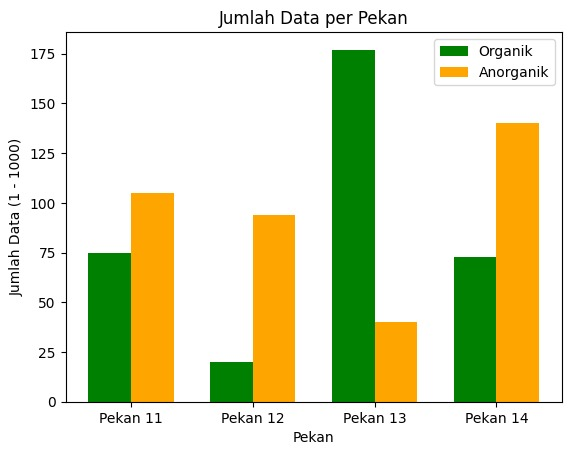
\includegraphics[width=0.6\linewidth]{Images/jumlahdataset.jpeg}
        \caption*{Gambar 2. EDA Pengumpulan Dataset}
        \label{fig:dataset_collection}
    \end{figure}
    \begin{itemize}
        \item \textbf{Organik:} 
        \begin{itemize}
            \item Pekan 1: 75 gambar
            \item Pekan 2: 20 gambar
            \item Pekan 3: 177 gambar
            \item Pekan 4: 73 gambar
            \item \textbf{Total:} 345 gambar
        \end{itemize}
        \item \textbf{Anorganik:}
        \begin{itemize}
            \item Pekan 1: 105 gambar
            \item Pekan 2: 94 gambar
            \item Pekan 3: 40 gambar
            \item Pekan 4: 140 gambar
            \item \textbf{Total:} 379 gambar
        \end{itemize}
    
    \end{itemize}

    \item \textbf{Total Dataset:} 724 gambar.
    \begin{figure}[h]
        \centering
        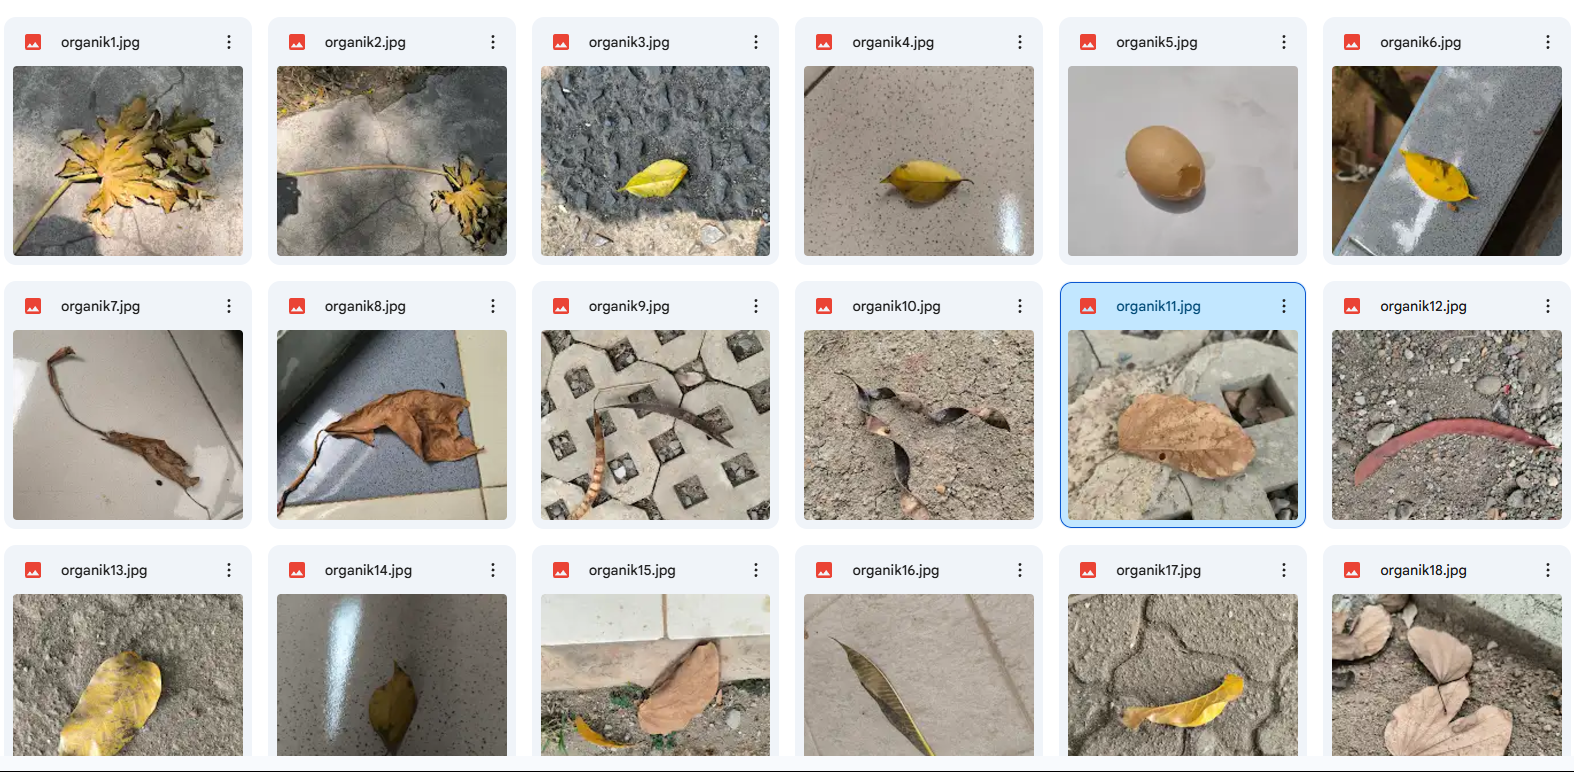
\includegraphics[width=0.6\linewidth]{Images/fotoorganik.png}
        \caption*{Gambar 3. Dataset Image Organik }
        \label{fig:dataset_collection}
    \end{figure}\begin{figure}[h]
        \centering
        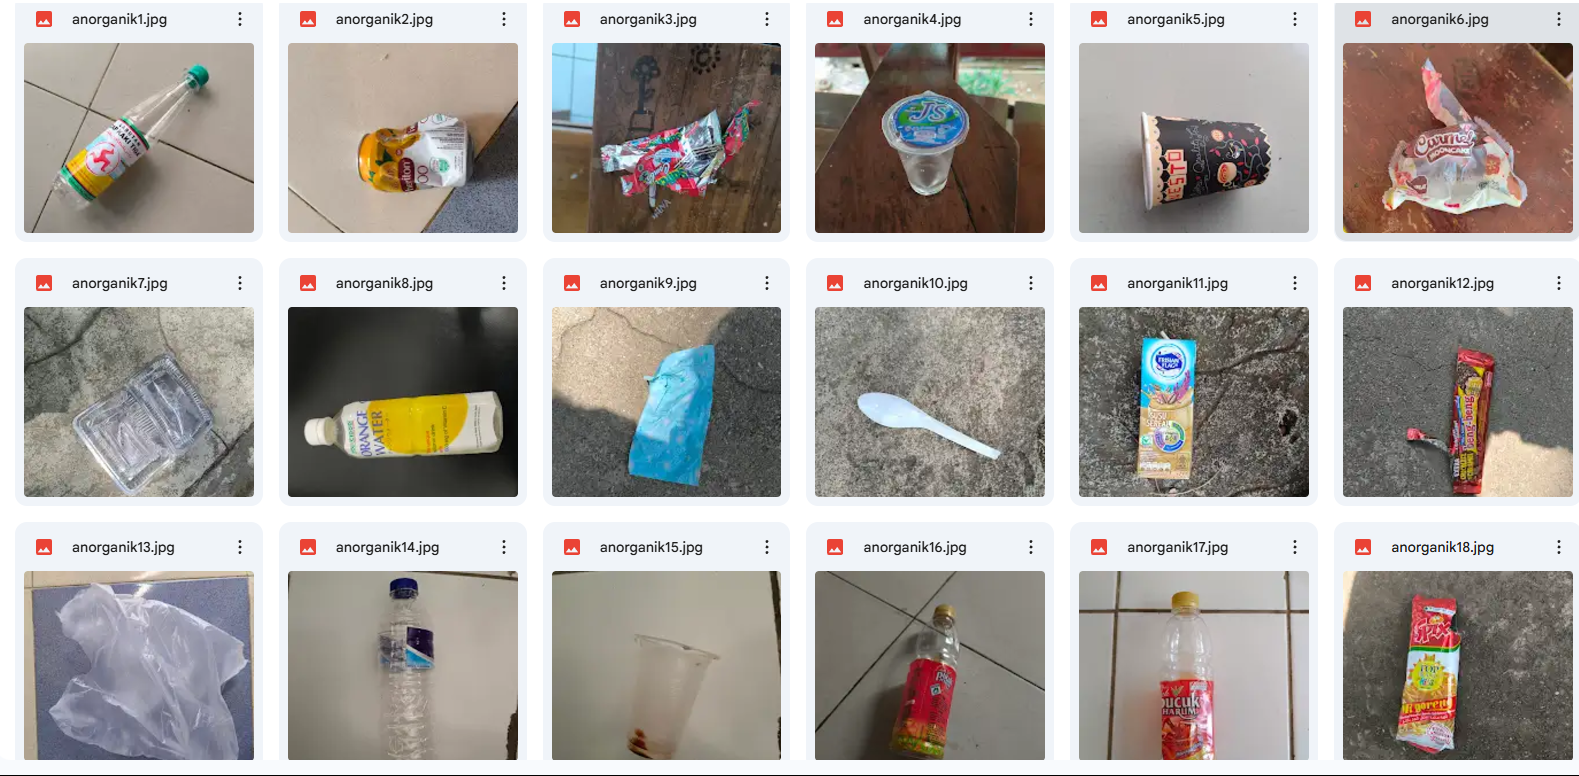
\includegraphics[width=0.6\linewidth]{Images/fotoanorganik.png}
        \caption*{Gambar 4. Dataset Image Anorganik}
        \label{fig:dataset_collection}
    \end{figure}

    \begin{figure}[H]
        \centering
        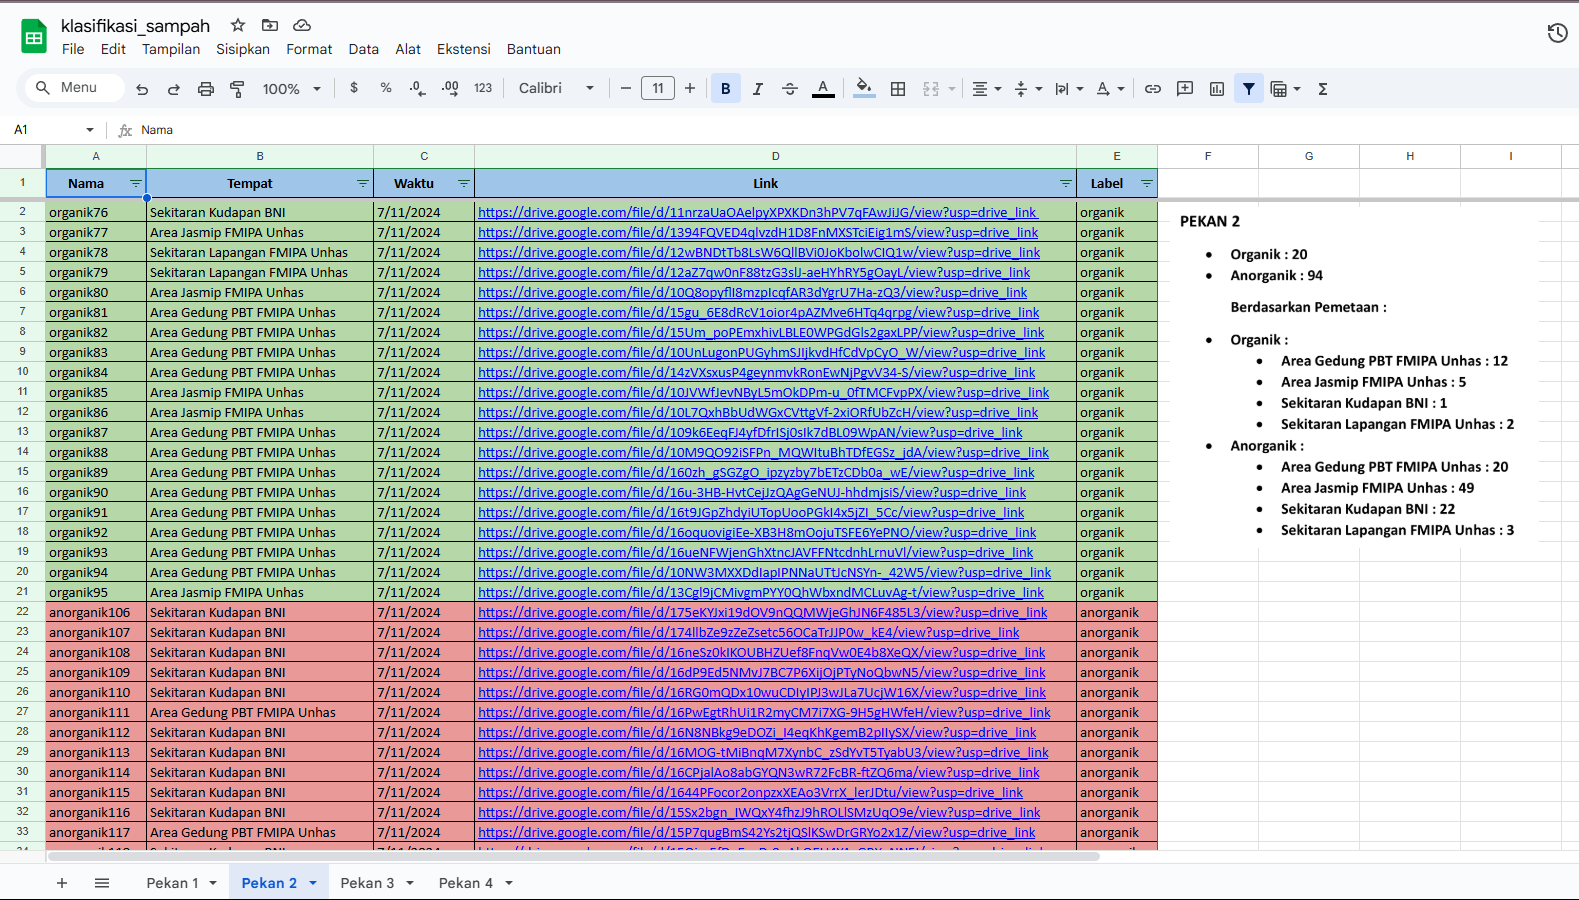
\includegraphics[width=0.6\linewidth]{Images/ss_excel.png}
        \caption*{Gambar 5. Dataset Dalam Excel}
        \label{fig:dataset_collection}
    \end{figure}

    Semua Dataset termasuk klasifikasi, lokasi pengambilan data, link data dalam drive sudah terangkum di dalam file excel
    
    \item \textbf{Proporsi Data Berdasarkan Label:}
    \begin{itemize}
        \item \textbf{Organik:} \(\frac{345}{724} \approx 47.65\%\)
        \item \textbf{Anorganik:} \(\frac{379}{724} \approx 52.35\%\)
    \end{itemize}

    \item \textbf{Format File:} Semua gambar disimpan dalam format JPG dengan ukuran 1:1. 
\end{itemize}

\subsection{Material dan Alat}

\subsubsection{Alat dan Platform Anotasi}
\begin{itemize}
    \item \textbf{Kamera Smartphone:} Digunakan untuk mengambil gambar sampah di berbagai lokasi di lingkungan Universitas Hasanuddin.
    \item \textbf{Google Colab:} Digunakan untuk pelatihan model dengan memanfaatkan GPU gratis yang disediakan, memungkinkan proses pelatihan yang lebih cepat dan efisien.
\end{itemize}

\subsubsection{Pustaka dan Kerangka Kerja}
\begin{itemize}
    \item \textbf{TensorFlow dan Keras:} Digunakan untuk membangun dan melatih model deep learning, termasuk arsitektur VGG16 dan ResNet.
    \item \textbf{OpenCV:} Digunakan untuk preprocessing gambar, seperti resize dan augmentasi.
    \item \textbf{Numpy dan Pandas:} Digunakan untuk manipulasi data dan analisis dataset, memudahkan pengolahan data dalam format array dan tabel.
    \item \textbf{Matplotlib dan Seaborn:} Digunakan untuk visualisasi data dan hasil pelatihan model, termasuk plot learning curve dan confusion matrix.
\end{itemize}


\section{RESULT AND DISCUSSION}
\subsection{Performance Metrics}

\begin{table}[H]
\centering
\begin{tabular}{|l|c|c|c|}
    \hline
    \textbf{Class} & \textbf{Precision} & \textbf{Recall} & \textbf{F1 Score} \\
    \hline
    Organik & 0.61 & 0.67 & 0.64 \\
    Anorganik & 0.46 & 0.4 & 0.43 \\
    \hline
\end{tabular}
\caption{Classification Report ResNet Pekan 1.}
\label{tab:resnet_week1}
\end{table}

\begin{table}[H]
\centering
\begin{tabular}{|l|c|c|c|}
    \hline
    \textbf{Class} & \textbf{Precision} & \textbf{Recall} & \textbf{F1 Score} \\
    \hline
    Organik & 0.63 & 0.57 & 0.6 \\
    Anorganik & 0.47 & 0.53 & 0.5 \\
    \hline
\end{tabular}
\caption{Classification Report VGG16 Pekan 1.}
\label{tab:vgg16_week1}
\end{table}

\begin{table}[H]
\centering
\begin{tabular}{|l|c|c|c|}
    \hline
    \textbf{Class} & \textbf{Precision} & \textbf{Recall} & \textbf{F1 Score} \\
    \hline
    Organik & 0.67 & 1 & 0.8 \\
    Anorganik & 0 & 0 & 0 \\
    \hline
\end{tabular}
\caption{Classification Report ResNet Pekan 2.}
\label{tab:resnet_week2}
\end{table}

\begin{table}[H]
\centering
\begin{tabular}{|l|c|c|c|}
    \hline
    \textbf{Class} & \textbf{Precision} & \textbf{Recall} & \textbf{F1 Score} \\
    \hline
    Organik & 0.74 & 0.79 & 0.77 \\
    Anorganik & 0.5 & 0.42 & 0.46 \\
    \hline
\end{tabular}
\caption{Classification Report VGG16 Pekan 2.}
\label{tab:vgg16_week2}
\end{table}

\begin{table}[H]
\centering
\begin{tabular}{|l|c|c|c|}
    \hline
    \textbf{Class} & \textbf{Precision} & \textbf{Recall} & \textbf{F1 Score} \\
    \hline
    Organik & 0.45 & 0.43 & 0.44 \\
    Anorganik & 0.53 & 0.56 & 0.54 \\
    \hline
\end{tabular}
\caption{Classification Report ResNet Pekan 3.}
\label{tab:resnet_week3}
\end{table}

\begin{table}[H]
\centering
\begin{tabular}{|l|c|c|c|}
    \hline
    \textbf{Class} & \textbf{Precision} & \textbf{Recall} & \textbf{F1 Score} \\
    \hline
    Organik & 0.49 & 0.51 & 0.5 \\
    Anorganik & 0.56 & 0.54 & 0.55 \\
    \hline
\end{tabular}
\caption{Classification Report VGG16 Pekan 3.}
\label{tab:vgg16_week3}
\end{table}

\begin{table}[H]
\centering
\begin{tabular}{|l|c|c|c|}
    \hline
    \textbf{Class} & \textbf{Precision} & \textbf{Recall} & \textbf{F1 Score} \\
    \hline
    Organik & 0.55 & 0.43 & 0.48 \\
    Anorganik & 0.5 & 0.62 & 0.55 \\
    \hline
\end{tabular}
\caption{Classification Report ResNet Pekan 4 / keseluruhan Dataset.}
\label{tab:resnet_week4}
\end{table}

\begin{table}[H]
\centering
\begin{tabular}{|l|c|c|c|}
    \hline
    \textbf{Class} & \textbf{Precision} & \textbf{Recall} & \textbf{F1 Score} \\
    \hline
    Organik & 0.52 & 0.57 & 0.55 \\
    Anorganik & 0.48 & 0.43 & 0.46 \\
    \hline
\end{tabular}
\caption{Classification Report VGG16 Pekan 4 / keseluruhan Dataset.}
\label{tab:vgg16_week4}
\end{table}

Berdasarkan hasil classification report yang ditunjukkan pada tabel \ref{tab:resnet_week1} hingga \ref{tab:vgg16_week4}, terlihat variasi performa yang menarik dari kedua model di setiap pekannya. Pada pekan pertama, model ResNet menunjukkan performa yang cukup baik untuk klasifikasi sampah organik dengan F1-score mencapai 0.64, sementara untuk sampah anorganik mencapai 0.43. Di sisi lain, model VGG16 menunjukkan performa yang lebih seimbang dengan F1-score 0.6 untuk organik dan 0.5 untuk anorganik. Hal ini mengindikasikan bahwa pada tahap awal, VGG16 lebih baik dalam menyeimbangkan klasifikasi antara kedua kelas.

Memasuki pekan kedua, terjadi fenomena yang menarik dimana model ResNet mengalami kesulitan serius dalam mengklasifikasikan sampah anorganik, terlihat dari F1-score yang mencapai 0, meskipun berhasil mencapai F1-score 0.8 untuk sampah organik. Sebaliknya, VGG16 menunjukkan peningkatan yang signifikan dengan F1-score 0.77 untuk organik dan 0.46 untuk anorganik. Peningkatan precision VGG16 menjadi 0.74 untuk kelas organik menunjukkan bahwa model ini semakin akurat dalam prediksi positifnya.

Pada pekan ketiga, kedua model menunjukkan perkembangan yang berbeda. ResNet berhasil mencapai keseimbangan yang lebih baik dengan F1-score 0.44 untuk organik dan 0.54 untuk anorganik. VGG16 juga menunjukkan performa yang seimbang dengan F1-score 0.5 untuk organik dan 0.55 untuk anorganik. Ini menandakan bahwa kedua model mulai beradaptasi dengan lebih baik dalam mengenali karakteristik kedua jenis sampah.

Di pekan keempat, yang mencakup keseluruhan dataset, ResNet mencatat F1-score 0.48 untuk organik dan 0.55 untuk anorganik, sementara VGG16 mencapai 0.55 untuk organik dan 0.46 untuk anorganik. Meskipun angka-angka ini menunjukkan performa yang cukup seimbang, nilai precision dan recall yang masih berkisar di angka 0.5 mengindikasikan bahwa masih ada ruang yang signifikan untuk peningkatan performa kedua model.


\begin{table}[H]
\centering
\begin{tabular}{|c|c|c|}
    \hline
    & \textbf{Predicted Organik} & \textbf{Predicted Anorganik} \\
    \hline
    \textbf{Actual Organik} & 14 & 7 \\
    \hline
    \textbf{Actual Anorganik} & 9 & 6 \\
    \hline
\end{tabular}
\caption{Confusion Matrix ResNet Pekan 1.}
\end{table}

\begin{table}[H]
\centering
\begin{tabular}{|c|c|c|}
    \hline
    & \textbf{Predicted Organik} & \textbf{Predicted Anorganik} \\
    \hline
    \textbf{Actual Organik} & 12 & 9 \\
    \hline
    \textbf{Actual Anorganik} & 7 & 8 \\
    \hline
\end{tabular}
\caption{Confusion Matrix VGG16 Pekan 1.}
\end{table}


\begin{table}[H]
\centering
\begin{tabular}{|c|c|c|}
    \hline
    & \textbf{Predicted Organik} & \textbf{Predicted Anorganik} \\
    \hline
    \textbf{Actual Organik} & 39 & 0 \\
    \hline
    \textbf{Actual Anorganik} & 19 & 0 \\
    \hline
\end{tabular}
\caption{Confusion Matrix ResNet Pekan 2.}
\end{table}

\begin{table}[H]
\centering
\begin{tabular}{|c|c|c|}
    \hline
    & \textbf{Predicted Organik} & \textbf{Predicted Anorganik} \\
    \hline
    \textbf{Actual Organik} & 31 & 8 \\
    \hline
    \textbf{Actual Anorganik} & 11 & 8 \\
    \hline
\end{tabular}
\caption{Confusion Matrix VGG16 Pekan 2.}
\end{table}


\begin{table}[H]
\centering
\begin{tabular}{|c|c|c|}
    \hline
    & \textbf{Predicted Organik} & \textbf{Predicted Anorganik} \\
    \hline
    \textbf{Actual Organik} & 20 & 27 \\
    \hline
    \textbf{Actual Anorganik} & 24 & 30 \\
    \hline
\end{tabular}
\caption{Confusion Matrix ResNet Pekan 3.}
\end{table}

\begin{table}[H]
\centering
\begin{tabular}{|c|c|c|}
    \hline
    & \textbf{Predicted Organik} & \textbf{Predicted Anorganik} \\
    \hline
    \textbf{Actual Organik} & 24 & 23 \\
    \hline
    \textbf{Actual Anorganik} & 25 & 29 \\
    \hline
\end{tabular}
\caption{Confusion Matrix VGG16 Pekan 3.}
\end{table}


\begin{table}[H]
\centering
\begin{tabular}{|c|c|c|}
    \hline
    & \textbf{Predicted Organik} & \textbf{Predicted Anorganik} \\
    \hline
    \textbf{Actual Organik} & 32 & 43 \\
    \hline
    \textbf{Actual Anorganik} & 26 & 43 \\
    \hline
\end{tabular}
\caption{Confusion Matrix ResNet Pekan 4.}
\end{table}

\begin{table}[H]
\centering
\begin{tabular}{|c|c|c|}
    \hline
    & \textbf{Predicted Organik} & \textbf{Predicted Anorganik} \\
    \hline
    \textbf{Actual Organik} & 43 & 32 \\
    \hline
    \textbf{Actual Anorganik} & 39 & 30 \\
    \hline
\end{tabular}
\caption{Confusion Matrix VGG16 Pekan 4.}
\end{table}

Analisis confusion matrix memberikan gambaran yang lebih detail tentang pola kesalahan klasifikasi kedua model. Pada pekan pertama, dari 21 sampel organik, ResNet berhasil mengklasifikasikan 14 dengan benar dan salah mengklasifikasikan 7 sampel. Untuk sampah anorganik, hanya 6 dari 15 sampel yang berhasil diklasifikasikan dengan benar. VGG16 menunjukkan pola serupa dengan 12 prediksi benar untuk organik dari 21 sampel, dan 8 prediksi benar untuk anorganik dari 15 sampel.

Pekan kedua menunjukkan fenomena yang unik dimana ResNet mengklasifikasikan seluruh sampel sebagai organik, menghasilkan 39 prediksi benar untuk organik tetapi gagal total dalam mengklasifikasikan 19 sampel anorganik. VGG16 menunjukkan performa yang lebih baik dengan 31 prediksi benar untuk organik dan 8 untuk anorganik, meskipun masih menunjukkan bias terhadap kelas organik.

Pada pekan ketiga, kedua model menunjukkan peningkatan dalam hal keseimbangan klasifikasi. ResNet mencapai 20 prediksi benar untuk organik dan 30 untuk anorganik, sementara VGG16 mencatat 24 prediksi benar untuk organik dan 29 untuk anorganik. Ini menunjukkan perkembangan positif dalam kemampuan model untuk mengenali karakteristik sampah anorganik.

Di pekan terakhir, yang mencakup dataset keseluruhan, ResNet berhasil mengklasifikasikan dengan benar 32 dari 75 sampel organik dan 43 dari 69 sampel anorganik. VGG16 mencapai 43 prediksi benar untuk organik dan 30 untuk anorganik. Meskipun ada peningkatan dalam jumlah prediksi yang benar, jumlah kesalahan klasifikasi yang masih signifikan menunjukkan kompleksitas dalam membedakan kedua jenis sampah.

\begin{table}[H]
\centering
\begin{tabular}{|l|c|c|}
    \hline
    \textbf{Model} & \textbf{Validation Accuracy} & \textbf{Validation Loss} \\
    \hline
    ResNet & 0.7222 & 0.645 \\
    \hline
    VGG16 & 0.8889 & 0.3515 \\
    \hline
\end{tabular}
\caption{Validation Accuracy and Loss Models Pekan 1}
\end{table}

\begin{table}[H]
\centering
\begin{tabular}{|l|c|c|}
    \hline
    \textbf{Model} & \textbf{Validation Accuracy} & \textbf{Validation Loss} \\
    \hline
    ResNet & 0.6724 & 0.6702 \\
    \hline
    VGG16 & 0.8103 & 0.3302 \\
    \hline
\end{tabular}
\caption{Validation Accuracy and Loss Models Pekan 2}
\end{table}


\begin{table}[H]
\centering
\begin{tabular}{|l|c|c|}
    \hline
    \textbf{Model} & \textbf{Validation Accuracy} & \textbf{Validation Loss} \\
    \hline
    ResNet & 0.703 & 0.6579 \\
    \hline
    VGG16 & 0.8713 & 0.2946 \\
    \hline
\end{tabular}
\caption{Validation Accuracy and Loss Models Pekan 3}
\end{table}


\begin{table}[H]
\centering
\begin{tabular}{|l|c|c|}
    \hline
    \textbf{Model} & \textbf{Validation Accuracy} & \textbf{Validation Loss} \\
    \hline
    ResNet & 0.6319 & 0.6724 \\
    \hline
    VGG16 & 0.9028 & 0.2597 \\
    \hline
\end{tabular}
\caption{Validation Accuracy and Loss Models Pekan 4 / Keseluruhan}
\end{table}


Hasil validasi dari model ResNet dan VGG16 selama empat pekan menunjukkan variasi yang signifikan dalam hal akurasi dan loss. Berikut adalah analisis rinci dari hasil validasi yang ditunjukkan pada tabel:

\begin{itemize}
    \item \textbf{Pekan 1:} 
    \begin{itemize}
        \item ResNet mencapai akurasi validasi sebesar 72.22\% dengan loss 0.645. Ini menunjukkan bahwa model memiliki kemampuan yang cukup baik dalam memprediksi data validasi, meskipun masih ada ruang untuk perbaikan dalam mengurangi loss.
        \item VGG16 menunjukkan performa yang lebih baik dengan akurasi validasi 88.89\% dan loss 0.3515, menandakan bahwa model ini lebih efektif dalam menangani data validasi pada pekan pertama.
    \end{itemize}

    \item \textbf{Pekan 2:}
    \begin{itemize}
        \item ResNet mengalami sedikit penurunan akurasi menjadi 67.24\% dengan loss 0.6702, yang menunjukkan bahwa model mungkin mengalami overfitting atau kesulitan dalam generalisasi.
        \item VGG16 tetap menunjukkan performa yang kuat dengan akurasi 81.03\% dan penurunan loss menjadi 0.3302, mengindikasikan peningkatan dalam kemampuan model untuk memprediksi data validasi dengan lebih baik.
    \end{itemize}

    \item \textbf{Pekan 3:}
    \begin{itemize}
        \item ResNet sedikit meningkat dalam akurasi validasi menjadi 70.3\% dengan loss 0.6579, menunjukkan perbaikan dalam generalisasi model.
        \item VGG16 terus menunjukkan performa yang unggul dengan akurasi 87.13\% dan penurunan loss lebih lanjut menjadi 0.2946, menandakan bahwa model ini semakin stabil dan efektif.
    \end{itemize}

    \item \textbf{Pekan 4 (Keseluruhan Dataset):}
    \begin{itemize}
        \item ResNet mengalami penurunan akurasi menjadi 63.19\% dengan loss 0.6724, yang mungkin disebabkan oleh kompleksitas dataset keseluruhan yang lebih tinggi.
        \item VGG16 mencapai akurasi tertinggi sebesar 90.28\% dengan loss terendah 0.2597, menunjukkan bahwa model ini sangat efektif dalam menangani dataset yang lebih besar dan kompleks.
    \end{itemize}
\end{itemize}

Secara keseluruhan, hasil validasi menunjukkan bahwa model VGG16 secara konsisten berkinerja lebih baik dari ResNet dalam hal akurasi dan loss, menandakan bahwa VGG16 lebih mampu dalam menangani variasi data dan mengurangi kesalahan prediksi. Namun, penurunan performa ResNet pada dataset keseluruhan menunjukkan perlunya optimasi lebih lanjut, seperti penyesuaian hyperparameter atau peningkatan teknik augmentasi data, untuk meningkatkan kemampuan generalisasi model.


\subsection{Visualization of Results}
\begin{adjustwidth}{3em}{0pt}

\begin{figure}[H]
    \centering
    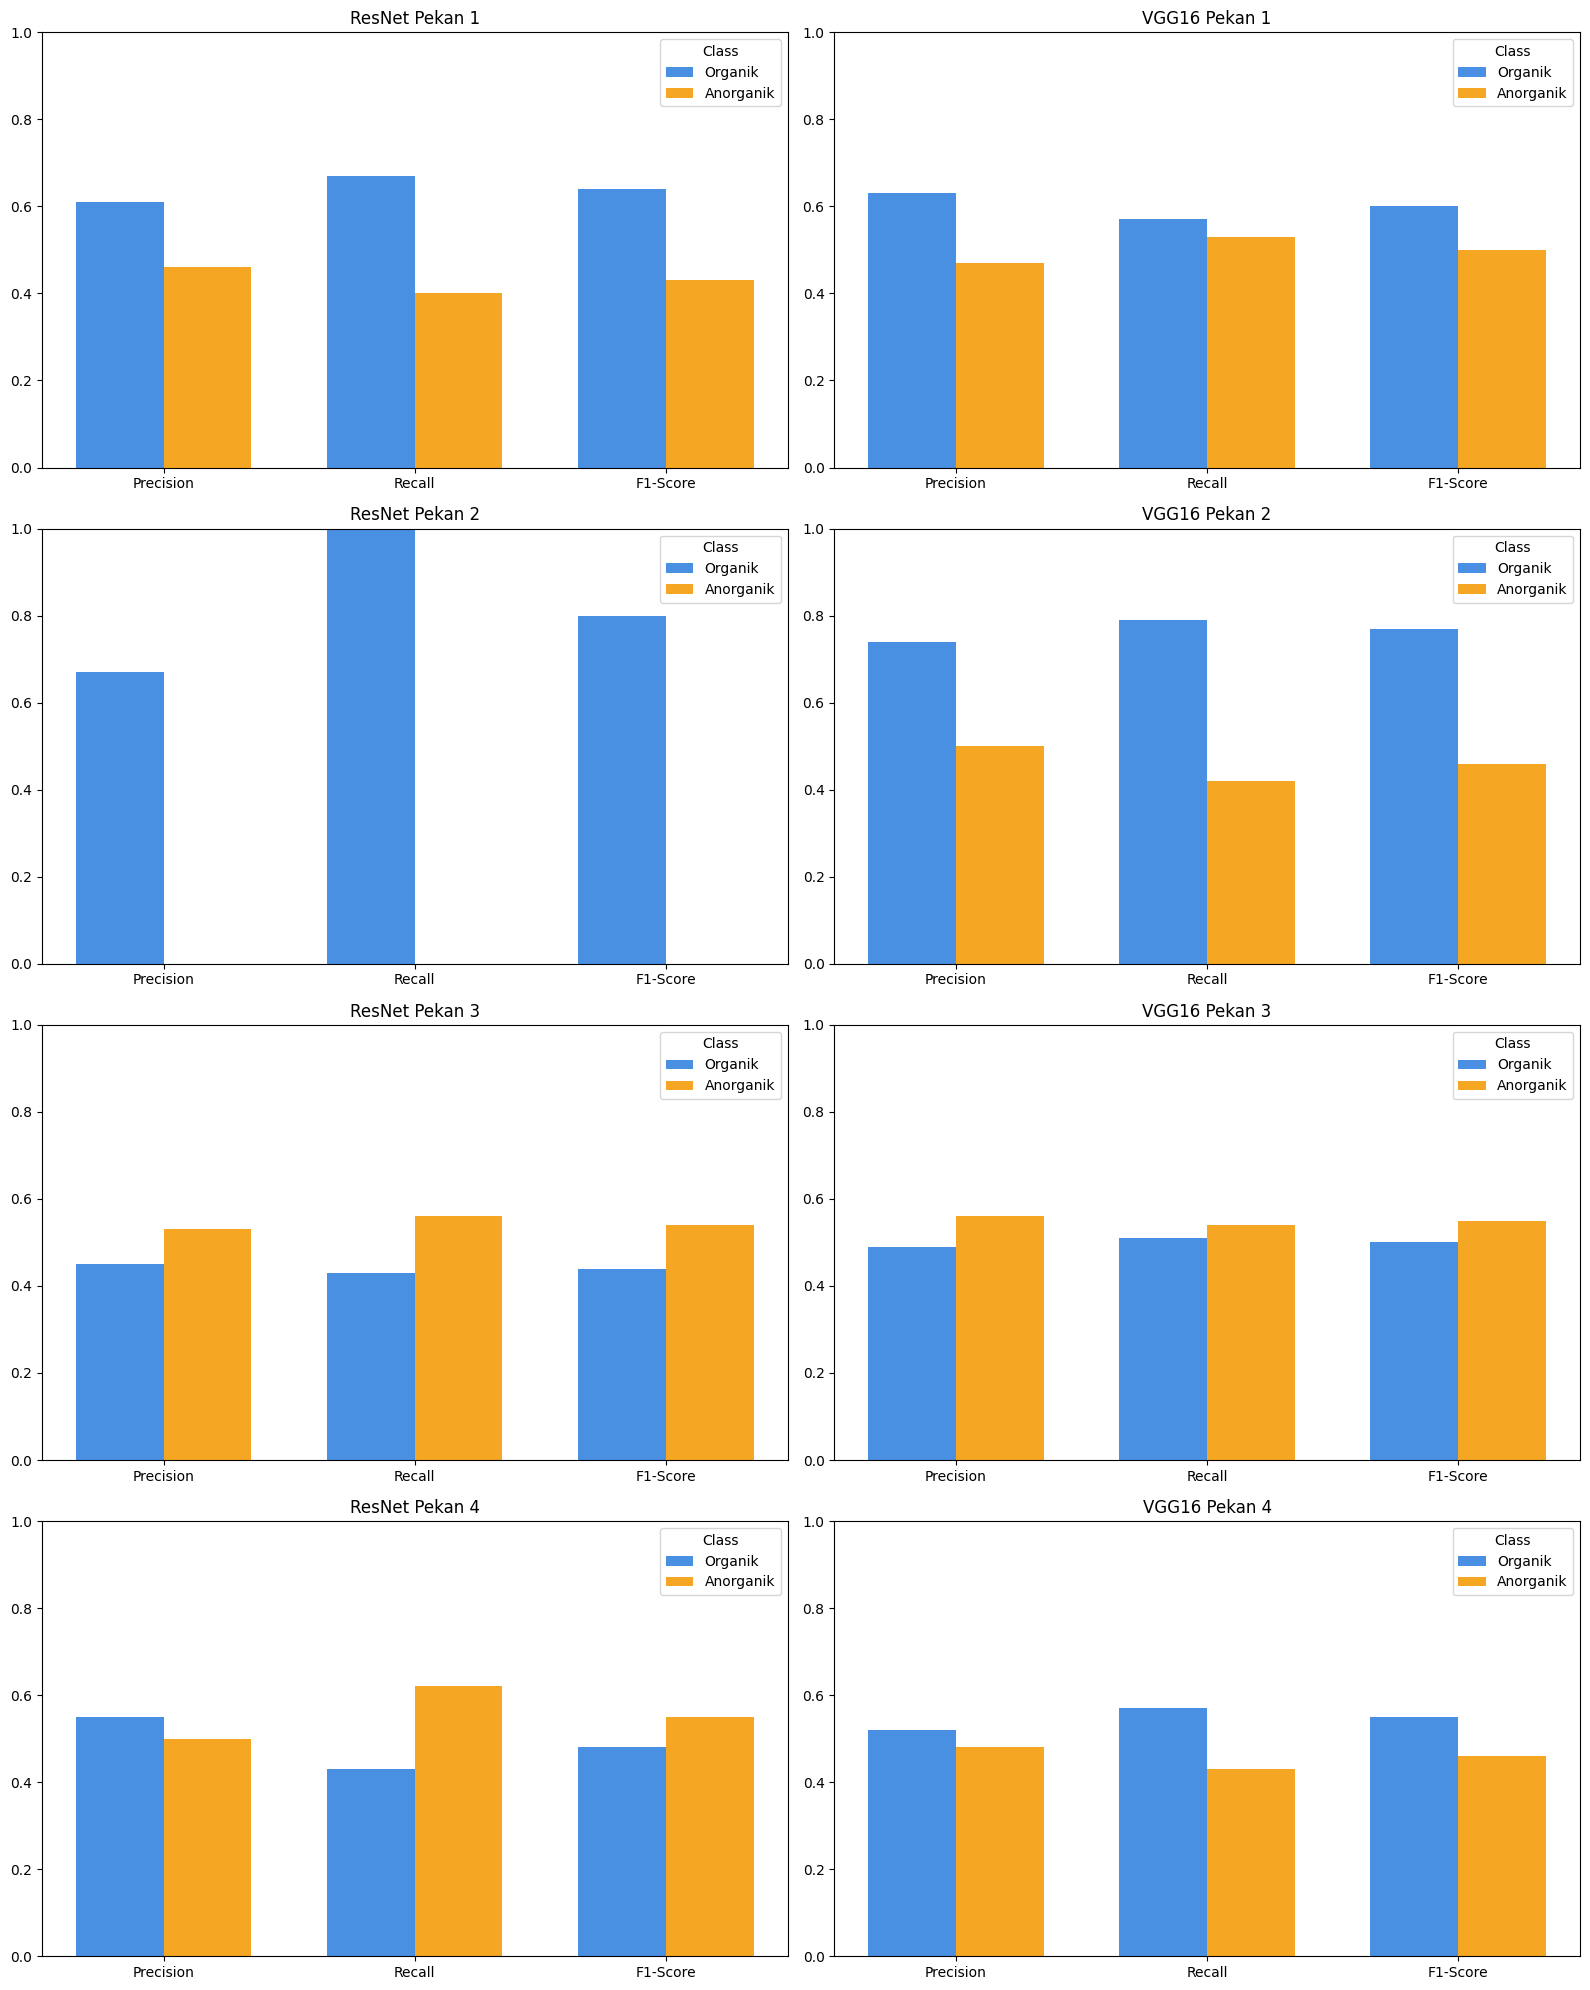
\includegraphics[width=1\linewidth]{Images/classificationreport.png}
    \caption*{Gambar 6. Classification Report Semua Pekan}
    \label{fig:dataset_collection}
\end{figure}

\begin{figure}[H]
    \centering
    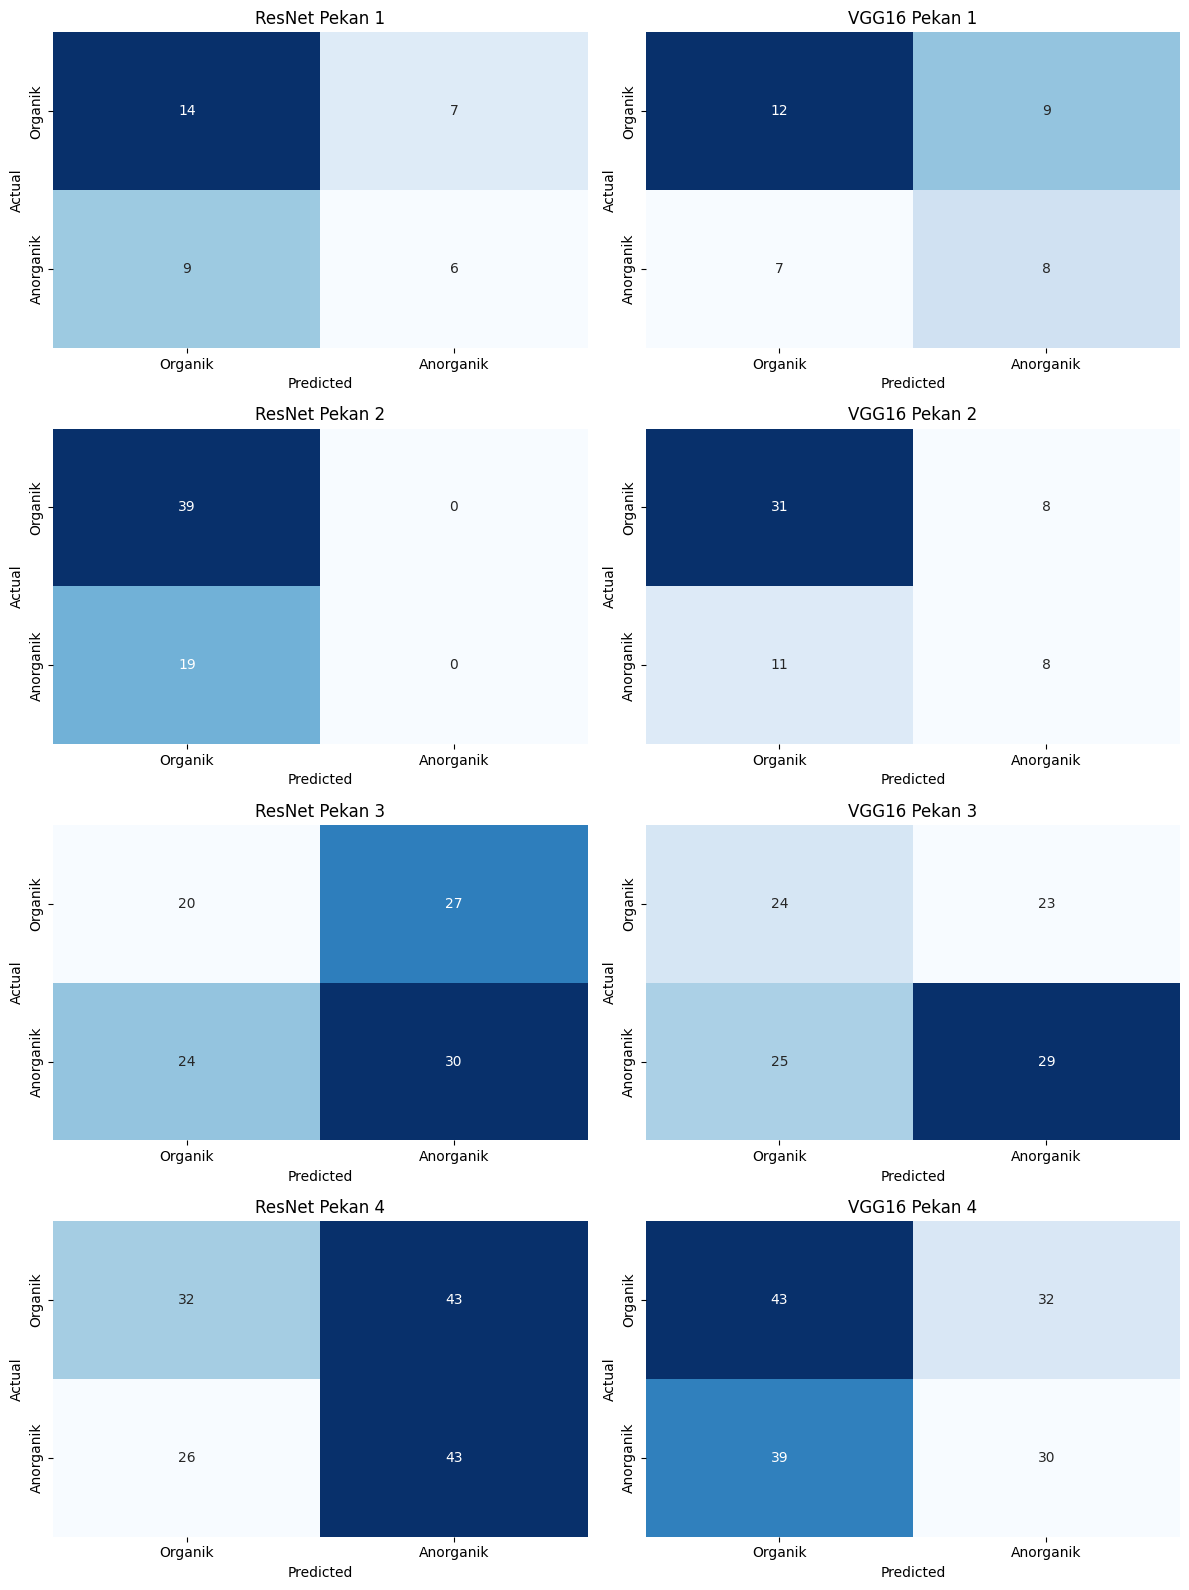
\includegraphics[width=1\linewidth]{Images/confusionmatrix.png}
    \caption*{Gambar 7. Confusion Matrix Semua Pekan}
    \label{fig:dataset_collection}
\end{figure}

\begin{figure}[H]
    \centering
    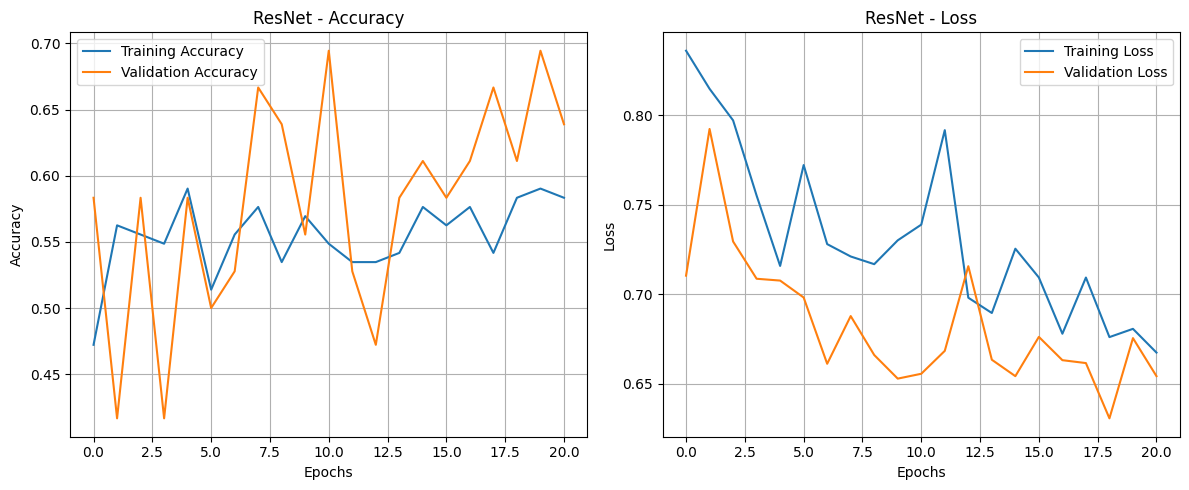
\includegraphics[width=1\linewidth]{Images/akurasipekan1resnet.png}
    \caption*{Gambar 8.  ResNet Accuracy Pekan 1}
    \label{fig:dataset_collection}
\end{figure}

\begin{figure}[H]
    \centering
    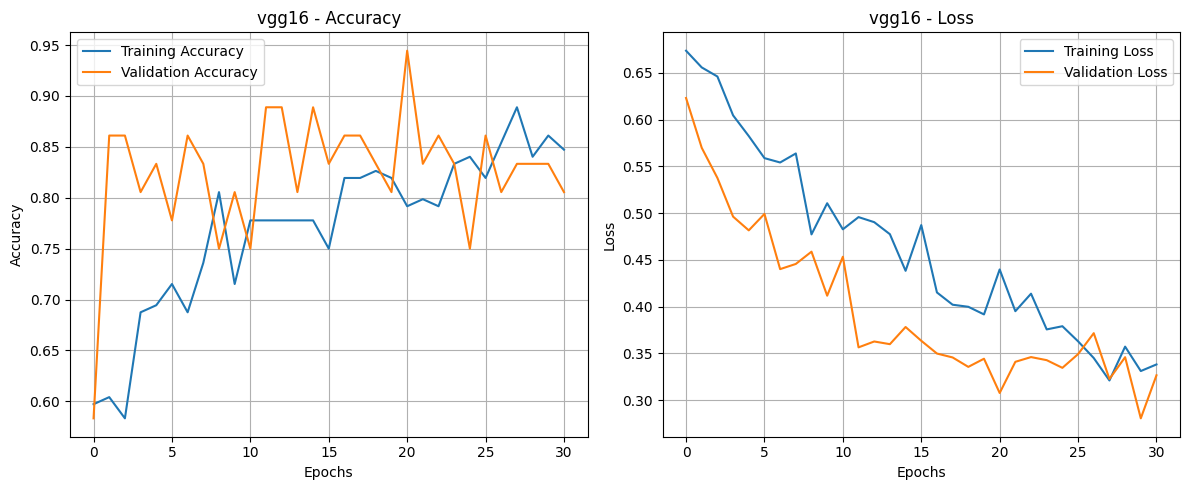
\includegraphics[width=1\linewidth]{Images/akurasipekan1vgg16.png}
    \caption*{Gambar 9.  vgg16 Accuracy Pekan 1}
    \label{fig:dataset_collection}
\end{figure}

\begin{figure}[H]
    \centering
    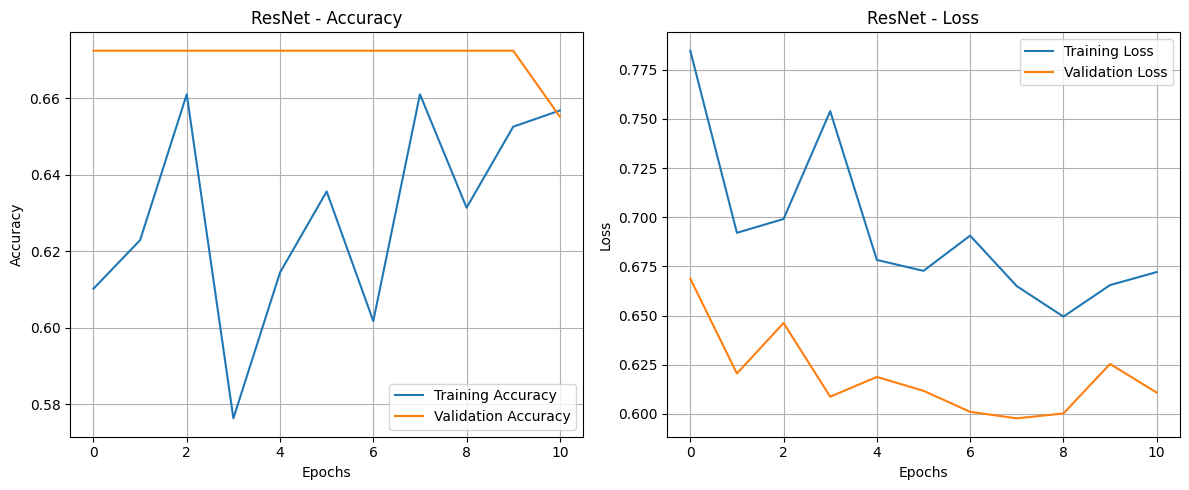
\includegraphics[width=1\linewidth]{Images/akurasipekan2resnet.png}
    \caption*{Gambar 10.  ResNet Accuracy Pekan 2}
    \label{fig:dataset_collection}
\end{figure}

\begin{figure}[H]
    \centering
    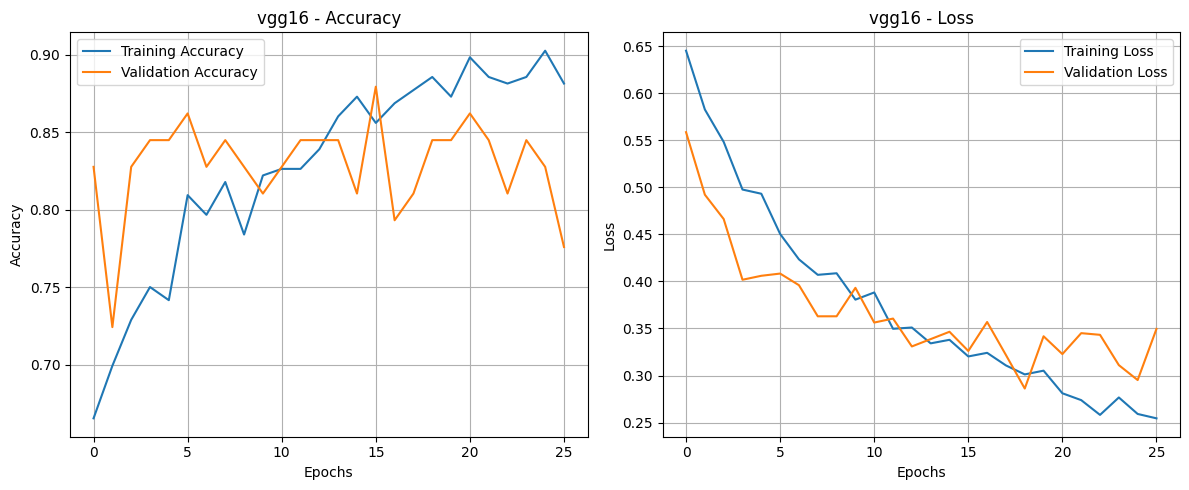
\includegraphics[width=1\linewidth]{Images/akurasipekan2vgg.png}
    \caption*{Gambar 11. vgg16 Accuracy Pekan 2}
    \label{fig:dataset_collection}
\end{figure}

\begin{figure}[H]
    \centering
    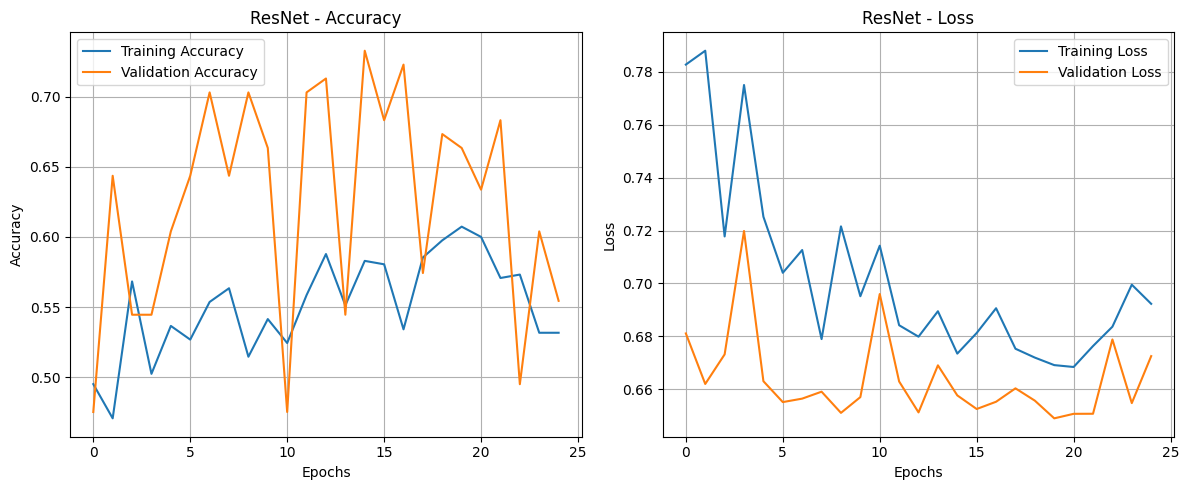
\includegraphics[width=1\linewidth]{Images/akurasipekan3resnet.png}
    \caption*{Gambar 12.  ResNet Accuracy Pekan 3}
    \label{fig:dataset_collection}
\end{figure}

\begin{figure}[H]
    \centering
    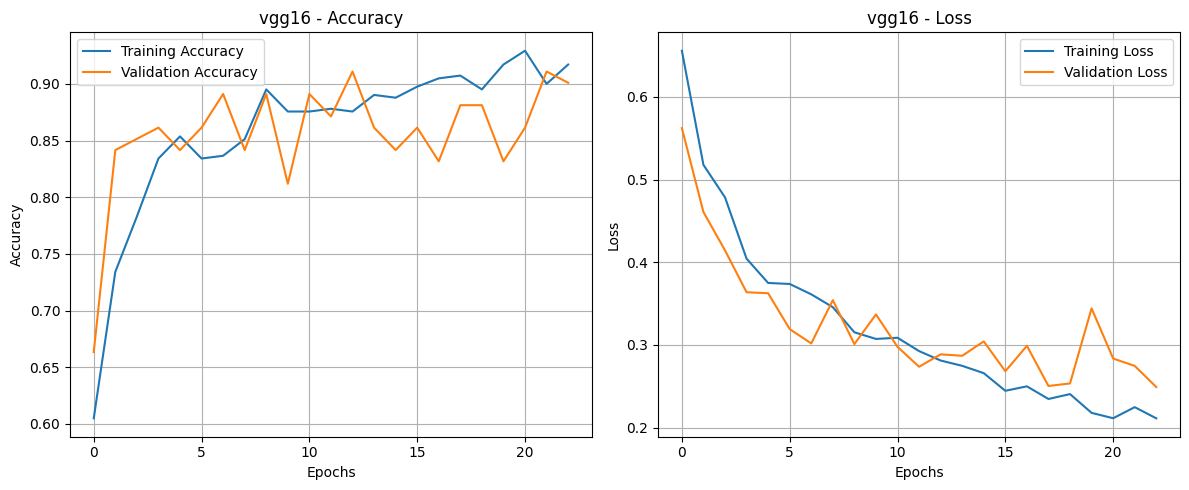
\includegraphics[width=1\linewidth]{Images/akurasipekan3vgg.png}
    \caption*{Gambar 13.  vgg16 Accuracy Pekan 3}
    \label{fig:dataset_collection}
\end{figure}

\begin{figure}[H]
    \centering
    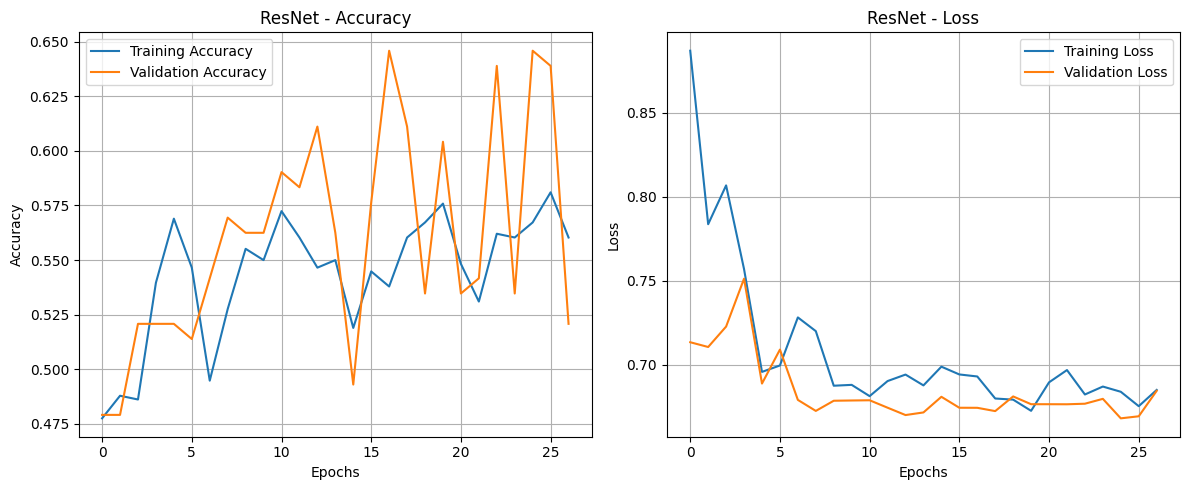
\includegraphics[width=1\linewidth]{Images/akurasipekan4resnet.png}
    \caption*{Gambar 14.  ResNet Accuracy Pekan 4}
    \label{fig:dataset_collection}
\end{figure}

\begin{figure}[H]
    \centering
    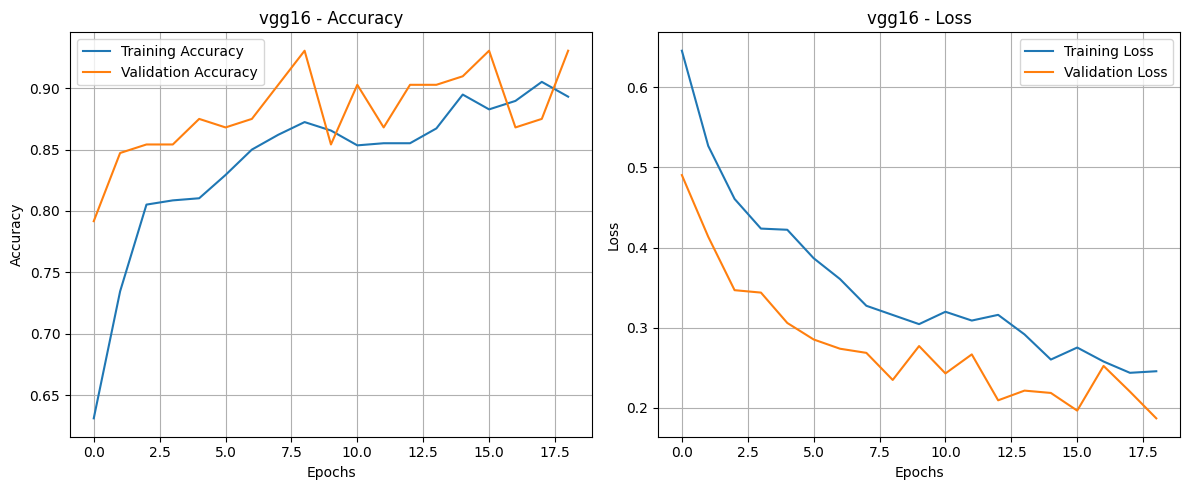
\includegraphics[width=1\linewidth]{Images/akurasipekan4vgg.png}
    \caption*{Gambar 15.  vgg16 Accuracy Pekan 4}
    \label{fig:dataset_collection}
\end{figure}

\end{adjustwidth}
\subsection{Discussion of the Results}
\begin{adjustwidth}{3em}{0pt}

Hasil penelitian ini memberikan perspektif baru dalam konteks klasifikasi sampah organik dan anorganik menggunakan arsitektur deep learning, khususnya dalam lingkungan kampus. Model VGG16 dalam penelitian ini mencapai akurasi validasi tertinggi 90.28\%, mengungguli hasil penelitian Rasidi et al. (2022) yang mencapai akurasi 85\% menggunakan CNN konvensional. Pencapaian ini menunjukkan keunggulan arsitektur yang lebih kompleks dalam menangani variasi data sampah. Namun, performa ResNet dalam penelitian ini yang hanya mencapai akurasi 63.19\% masih jauh di bawah hasil Parasian (2022) yang mencapai akurasi validasi 96\% menggunakan ResNet50. Perbedaan signifikan ini kemungkinan disebabkan oleh variasi dalam implementasi transfer learning dan optimasi hyperparameter.

Dalam aspek metodologi dan tantangan, penelitian ini menghadapi masalah yang serupa dengan yang diidentifikasi oleh Sunanto (2022), di mana overfitting menjadi tantangan utama dalam klasifikasi sampah. Hal ini terlihat jelas pada performa ResNet di pekan kedua yang menunjukkan bias ekstrem terhadap kelas organik. Meskipun pendekatan berbasis computer vision kami tidak mencapai performa sebaik sistem multi-sensor Fantara et al. (2018) yang mencapai akurasi 90\%, metodologi kami menawarkan fleksibilitas dan skalabilitas yang lebih baik untuk implementasi praktis.

Konteks spesifik kampus memberikan karakteristik unik pada penelitian ini. Berbeda dengan penelitian Fathurrahman (2024) yang mencapai mAP 0.858, fokus kami pada lingkungan kampus menghadirkan tantangan tersendiri dalam hal variasi dan distribusi jenis sampah. Hal ini tercermin dari F1-score yang bervariasi antar pekan (0.43-0.8), menunjukkan kompleksitas dalam menangani sampah kampus yang memiliki pola penggunaan berbeda dari lingkungan umum.

Dari segi implementasi, meskipun tidak mencapai akurasi setinggi sistem real-time Priana dan Karyawati (2023) yang mencapai 80-100\%, pendekatan evaluasi mingguan dalam penelitian ini memberikan insight penting tentang evolusi performa model dalam konteks dataset yang berkembang. Pola adaptasi model yang terungkap melalui evaluasi berkala ini merupakan kontribusi unik yang belum banyak dibahas dalam penelitian sebelumnya, memberikan pemahaman lebih baik tentang stabilitas model dalam penggunaan jangka panjang.

Penelitian ini memberikan kontribusi signifikan dengan menyajikan analisis komparatif mendalam antara VGG16 dan ResNet dalam konteks spesifik sampah kampus, melengkapi studi-studi sebelumnya yang umumnya berfokus pada satu arsitektur. Temuan tentang superioritas VGG16 dalam konteks ini memberikan pertimbangan penting untuk pengembangan sistem klasifikasi sampah di lingkungan akademik. Meskipun beberapa aspek performa masih di bawah benchmark yang ditetapkan oleh penelitian sebelumnya, kontribusi unik penelitian ini terletak pada evaluasi komprehensif dalam konteks kampus dan analisis longitudinal yang memberikan wawasan berharga untuk pengembangan sistem klasifikasi sampah yang lebih efektif di lingkungan akademik.

\end{adjustwidth}



% 5. Conclusion
% 5. Conclusion
\section{CONCLUSION}
\begin{adjustwidth}{3em}{0pt}
\subsection{Rekap Tujuan dan Pencapaian}
\hspace{0.5cm} Penelitian ini telah berhasil mencapai tujuan utamanya dalam mengembangkan dataset komprehensif yang terdiri dari sampah organik dan anorganik dari lingkungan Universitas Hasanuddin. Pengumpulan data yang dilakukan secara bertahap selama empat pekan telah menghasilkan dataset yang representatif untuk konteks kampus. Implementasi dan evaluasi dua arsitektur CNN, yaitu VGG16 dan ResNet, telah dilakukan secara sistematis, dengan VGG16 menunjukkan performa superior mencapai akurasi validasi 90.28\% pada dataset keseluruhan. Analisis komparatif kedua model telah memberikan wawasan berharga tentang efektivitas masing-masing arsitektur dalam konteks klasifikasi sampah kampus.

\subsection{Wawasan Utama dari Hasil}
\hspace{0.5cm} Hasil penelitian mengungkapkan beberapa wawasan penting. VGG16 secara konsisten mengungguli ResNet dalam semua metrik evaluasi, dengan performa terbaik dicapai pada dataset keseluruhan (akurasi 90.28\%, loss 0.2597). Sebaliknya, ResNet menunjukkan keterbatasan dalam generalisasi, terutama terlihat dari penurunan performa pada dataset yang lebih besar (akurasi 63.19\%, loss 0.6724). Evaluasi mingguan mengungkapkan bahwa kedua model menunjukkan pola adaptasi yang berbeda terhadap pertambahan data, dengan VGG16 menunjukkan stabilitas yang lebih baik. Klasifikasi sampah anorganik secara umum lebih menantang dibandingkan sampah organik, terlihat dari F1-score yang lebih rendah untuk kategori anorganik di kedua model.

\subsection{Pekerjaan dan Rekomendasi di Masa Depan}
\hspace{0.5cm} Berdasarkan hasil penelitian, beberapa rekomendasi untuk pengembangan masa depan dapat diusulkan. Dalam hal pengembangan dataset, diperlukan perluasan dengan variasi yang lebih besar dalam kondisi pencahayaan dan sudut pengambilan gambar, serta penambahan sub-kategori untuk klasifikasi yang lebih spesifik. Optimasi model dapat dilakukan dengan mengeksplorasi teknik augmentasi data yang lebih advanced dan menerapkan teknik ensemble learning untuk mengkombinasikan kekuatan kedua model. Untuk implementasi praktis, pengembangan sistem real-time dengan optimasi untuk perangkat edge dan perancangan interface yang user-friendly menjadi prioritas untuk implementasi di berbagai lokasi kampus. Evaluasi lanjutan perlu dilakukan untuk menguji performa dalam kondisi operasional nyata dan menganalisis efektivitas sistem dalam mendukung program 3R kampus.

\hspace{0.5cm} Secara keseluruhan, penelitian ini telah meletakkan dasar yang kuat untuk pengembangan sistem klasifikasi sampah otomatis di lingkungan kampus. Meskipun masih ada ruang untuk perbaikan, hasil yang dicapai menunjukkan potensi signifikan untuk implementasi praktis dalam mendukung program pengelolaan sampah yang lebih efisien di Universitas Hasanuddin.

\end{adjustwidth}
\newpage
\begin{thebibliography}{99}
\begin{enumerate}
    \item A. I. Rasidi, Y. A. H. Pasaribu, A. Ziqri, and F. D. Adhinata, "Klasifikasi Sampah Organik dan Non-Organik Menggunakan Convolutional Neural Network," Jurnal Teknik Informatika dan Sistem Informasi, vol. 8, no. 1, Apr. 2022.

    \item S. Surianti, "Analisis Karakteristik Sampah Organik dan Anorganik Di Kota Baubau (Studi Kasus Kel. Tomba)," Jurnal Media Inovasi Teknik Sipil UNIDAYAN, vol. 11, no. 2, pp. 77–81, Oct. 2022.

    \item Pernando, M. R. Muttaqin, and Y. R. Ramadhan, "DETEKSI JENIS SAMPAH SECARA REALTIME MENGGUNAKAN METODE SINGLE SHOT MULTIBOX DETECTOR (SSD)," JATI (Jurnal Mahasiswa Teknik Informatika), vol. 7, no. 3, pp. 1890–1895, Nov. 2023.

    \item P. O. Parasian and F. Utaminingrum, "Rancang Bangun Sistem Pengklasifikasi Jenis Sampah Organik dan Sampah Daur Ulang menggunakan Resnet50," Jurnal Pengembangan Teknologi Informasi dan Ilmu Komputer, vol. 6, no. 2, pp. 727–732, 2022.

    \item A. A. Fathurrahman and F. Akbar, "Perancangan Sistem Identifikasi Jenis Sampah Menggunakan Tensorflow Object Detection Dan Transfer Learning," Jurnal Nasional Teknologi dan Sistem Informasi, vol. 10, no. 1, pp. 64–71, May 2024.

    \item F. P. Fantara, D. Syauqy, and G. E. Setyawan, "Implementasi Sistem Klasifikasi Sampah Organik dan Anorganik dengan Metode Jaringan Saraf Tiruan Backpropagation," Jurnal Pengembangan Teknologi Informasi dan Ilmu Komputer, vol. 2, no. 11, pp. 5577–5586, 2018.

    \item S. Wahyuningsih, B. Widiati, T. Melinda, and T. Abdullah, "Sosialisasi Pemilahan Sampah Organik dan Non-Organik Serta Pengadaan Tempat Sampah Organik dan Non-Organik," Dedikasi Saintek Jurnal Pengabdian Masyarakat, vol. 2, no. 1, pp. 7–15, Apr. 2023.

    \item O. Devi and P. H. Utomo, "IMPLEMENTASI DEEP LEARNING DENGAN CONVOLUTIONAL NEURAL NETWORK UNTUK KLASIFIKASI GAMBAR SAMPAH ORGANIK DAN ANORGANIK," UNEJ e-Proceeding, pp. 373–382, 2022.

\end{enumerate}
\end{thebibliography}
\end{document}